\newcommand{\lp}[1]{LP(\ensuremath{#1})}

\section{Correctness}
\label{sec:proof}

In order to lay out foundations  for reasoning about correctness,  we  define in Section~\ref{sec:spec} the model and correctness notion we seek to prove. 
We proceed to prove the algorithm's safety in Section~\ref{sec:safe} and liveness in Section~\ref{sec:live}.

\subsection{Model and Correctness Specification}
\label{sec:spec}

We consider an asynchronous shared memory model~\cite{Welch2004} consisting of a collection of shared variables accessed by a finite number of threads , which also have local state.
High-level objects, such as a map, are implemented using low-level memory objects supporting atomic read, write, and read-modify-write (e.g., CAS) primitives. 
Threads  \emph{invoke} high-level \emph{operations}, which perform a sequence of  \emph{steps} on low-level objects, and finally \emph{return}.

An \emph{algorithm} defines the behaviors of threads executing high-level operations as deterministic state machines, where local state transitions are associated with  shared low-level memory 
accesses (read, write, CAS, etc.) or high-level invocations/responses.
A \emph{configuration} describes the  local states of all threads and the contents of shared variables. An \emph{initial configuration} is one where all threads and variables  are in their initial values.
An \emph{execution} of algorithm $\mathcal{A}$ is an alternating sequence of configurations and steps, beginning with some initial configuration, 
such that configuration transitions occur according to $\mathcal{A}$.
Operation $op_1$ \emph{precedes} operation $op_2$ in an execution if $op_1$'s return step precedes $op_2$'s invoke step;
two operations are \emph{concurrent} in execution $\sigma$  if neither precedes the other, that is, both are invoked in $\sigma$  before either returns.
 In a  \emph{sequential} execution, there are no concurrent operations.
We use the notion of time \emph{t} during an execution $\sigma$  to refer to the configuration reached after the $t^{th}$ step in $\sigma$.
An \emph{interval} of execution $\sigma$ is a sub-sequence of $\sigma$.
The \emph{interval of an operation} $op$ in $\sigma$  starts with the invocation step of $op$ and ends with the configuration following the return from $op$ or 
the end of $\sigma$, if there is no such return.

Our correctness notion is \emph{linearizability}, which intuitively means that the object ``appears to be'' executing sequentially. 
More formally, the \emph{history} $H(\sigma)$ of execution $\sigma$ is the sequence of invocations  and returns occurring in $\sigma$. 
In a sequential history, each invocation is immediately followed by its return. 
An object is specified using a \emph{sequential specification}, which is the set of its allowed sequential histories. 

For a history $h$, \emph{complete($h$)} is the sequence obtained by removing invocations with no responses from $h$.
We assume that histories are \emph{well-formed}, meaning that the sub-sequence of each thread's steps in a history is sequential.
An algorithm is \emph{linearizable}~\cite{HerlihyW1990} if each of its histories $h=H(\sigma)$ can be extended by adding zero or more response events to a history $h'$, 
so that  \emph{complete($h'$)} has a sequential permutation that preserves $h$'s precedence relation and satisfies the object's sequential specification. 
Thus, a linearizable algorithm provides the illusion that each invoked operation takes effect instantaneously at some  \emph{linearization point} inside its interval. 

For liveness, we consider two notions: \emph{wait-freedom} requires that \emph{every} operation return within a finite number of its own steps, whereas \emph{lock-freedom}  
requires only that \emph{some} operation return within a finite number of steps. The former is sometimes called \emph{starvation-freedom} and the latter -- \emph{non-blocking}. 

\kiwi\ implements a linearizable map offering lock-free put operations and wait-free get and scan operations. 
In its sequential specification, get and scan return the latest value inserted by a put for each key in their ranges.





\subsection{\kiwi's Linearizability}
\label{sec:safe}

In Section~\ref{ssec:rebalance-proof} we show that the rebalance process preserves the data structure's integrity and contents. 
We proceed to prove that  {\kiwi} is linearizable by identifying, for every operation in a given execution, a {linearization point} between its invoke and return steps, so that the operation ``appears to'' occur atomically at this point.  We discuss put operations in Section~\ref{ssec:put-proof}, and gets and scans in Section~\ref{ssec:get-proof}. 
The linearization point of operation $op$ is denoted \lp{op}. 



\subsubsection{Rebalance.}
\label{ssec:rebalance-proof}

We first argue that rebalance operations preserve the integrity of the data structure.  
To this end, we introduce some definitions. 
We say that a chunk $C$ is \emph{accessible} in \kiwi\ if $C$ is connected to the linked list, 
that is, if traversing the linked list from its head to its tail goes through $C$. 
While a chunk is accessible its key range is well-defined: 
We say that key $k$ is in the \emph{range} of chunk $C$ if $k \geq C$.\code{minKey} and $k < C.$\code{next.minKey}.

When all the entries in a chunk's PPA are frozen, we say that the chunk is \emph{frozen}. 
Observe that a put operation can successfully assign a PPA version (phase 2 of put) in chunk $C$ at a time $t$ only if  (1) $C$ is accessible  at some time $t'<t$, 
and (2) $C$ is not frozen at time $t$. This is because once a thread's PPA entry is frozen, its attempt to CAS it inevitably fails and it triggers rebalance.
We say that a chunk is \emph{mutable} if these two conditions are satisfied. Similarly, a chunk is \emph{immutable} before it first becomes accessible 
and again after the freezing stage of its rebalance is complete. 

Rebalance preserves the following invariant:
\begin{invariant}
At any point in an execution of \kiwi, for every key $k$,  
\begin{enumerate}
\item the \code{minKey} values in the linked list are monotonically increasing (so $k$ is in the range of exactly one accessible chunk);  
\item  $k$ is in the range of at most one mutable chunk; and 
\item querying the index for $k$  returns a chunk $C$ s.t.\  $C$.\code{minKey} $\le k$ and $C$ is either accessible or frozen.
\end{enumerate}
\label{invariant:rebalance}
\end{invariant}
\begin{proof}
\begin{enumerate}
\item
Observe that when a segment of new chunks is connected instead of a sequence of old ones, $C_f$.\code{minKey} is equal to $C$.\code{minKey}, 
and  the \code{next} pointer in $C$'s predecessor is replaced via CAS from $C$ to $C_f$ (line~\ref{l:set-pred}) hence the invariant is preserved on the left side of the new segment.
The invariant is also preserved on the right side of the new segment because each new chunk's \code{minKey} is set to some key encountered in the old segment before \code{last}, 
and $C_n$.\code{next} is guaranteed to be \code{last.next} (lines  \ref{l:mark}--\ref{l:mark-end}).  
\item
The rebalance protocol does not link new chunks to the list (stage (5)) 
before freezing the old chunks holding the same key range (stage (2)).
Moreover, once a chunk is engaged (stage (1)), it is associated with a unique rebalance object \code{ro}
whose next pointer is set to $\bot$, 
and hence the segment of chunks associated with \code{ro} cannot change. 
Using a CAS to set $C$'s predecessor's \code{next} pointer to $C_f$ ensures 
that the old immutable chunk is replaced by at most one new accessible mutable chunk.
\item
Chunks are indexed according to their \code{minKey}, and 
the rebalance protocol does not index new chunks (stage (6)) before making them accessible (stage (5)). 
Before a chunk ceases to be accessible, it must be frozen. 
\end{enumerate}
\end{proof}

From Invariant~\ref{invariant:rebalance}, we derive the correct execution of the locate function:
\begin{corollary}
The locate(key) function  (lines~\ref{l:locate-start}-\ref{l:locate-end}) always returns a chunk $C$ s.t. key is in $C$'s range.
Moreover, if key is in the range of some chunk $C$ that is mutable throughout the execution of locate, then locate returns $C$.
\end{corollary}

In addition to preserving the data structure's integrity, rebalance ensures that no key-value pairs disappear from the data structure due to rebalancing. 
We say that a key-value pair $\langle$key, val$ \rangle$ is \emph{stored in} \kiwi\ at time $t$ in execution $\sigma$ if invoking get(key) at the end of $\sigma$
and allowing it to complete without interfering steps of other threads returns val. We show the following:

\begin{proposition}
If $\langle$key, val$ \rangle$ is \emph{stored in} \kiwi\ at time $t$ in execution $\sigma$ and no subsequent put(key,$\_$)  operations are invoked in $\sigma$, 
then $\langle$key, val$ \rangle$ is \emph{stored in} \kiwi\ at all times $t' > t$ in  $\sigma$.
\label{proposition:no-loss}
\end{proposition}
\begin{proof}
By Invariant~\ref{invariant:rebalance}(1), key is in the range of exactly one accessible chunk $C$ at time $t$,  which  get(key) locates, 
and the returned val is the one associated with key with the highest version (with ties broken by valPtr). 
Observe that as long as $C$ remains accessible at time $t'$, its range does not change because \code{minKey} is invariant, and if $C$'s successor is 
replaced by rebalance, it is replaced with a chunk with the same \code{minKey}. 
Since no   subsequent put(key,$\_$)  operations are invoked in $\sigma$, val remains the highest-version value associated with key in $C$, and we are done.

It remains to show that a rebalance that removes $C$ does not remove $\langle$key, val$ \rangle$ from \kiwi, from which the proposition follows   inductively.
%Consider therefore a rebalance that engages $C$.  %Once $C$.\code{ro} is set, it does not change.
This, in turn, follows from the facts that (1) the highest-versioned value associated with each key in an old chunk $C$ is cloned into a new chunk; and 
(2) the entire chunk segment is replaced atomically by first marking the next pointer of the last engaged chunk to prevent it from changing, and then 
CASing the predecessor of the first engaged chunk.
 \end{proof}

\subsubsection{Puts.} 
\label{ssec:put-proof}

Puts in a chunk $C$
are ordered (lexicographically) according to their version-value-index   pairs $\langle v, j \rangle$, where
$\langle v, i \rangle$ is published in the appropriate  PPA entry in phase 2 of the put, and \code{$C$.k[$i$].valPtr$=j$}; this pair is called the \emph{full version} of the put.
We note that in each chunk, the full versions are unique, because threads obtain $j$ using F\&A (line~\ref{l:put-cas-j}).
First,  $i$ is published in \code{ppa[t].idx} (line~\ref{l:put-version}) and then
the  pair gets its final value by a successful CAS of \code{ppa[t].ver}, either by the put (line~\ref{l:put-cas-version}) or by a helping thread (line~\ref {l:get-help}). 
We refer to 
a step publishing $i$ in \code{ppa[t].idx} and to
the step executing the successful CAS  as the put's \emph{publish time} and the \emph{full version assignment time}, resp., 
and say that the put \emph{assigns} full version $\langle v, j \rangle$ for its key in $C$.

We note that each put assigns a full version at most once. 
Furthermore, as noted above, a full version can only be assigned in a mutable chunk.
Once a put operation $po$ for key $k$ assigns its full version in chunk $C$ at time $t$, we can define its linearization point. 
There are two options: 
\begin{enumerate}
\item If at time $t$
$po$'s full version $\langle v, j \rangle$ is the highest for $k$ in $C$, (among entries in $C$'s {PPA} and  linked list),
then  \lp{po} is the last step (by any thread) that reads $v$ from \code{GV} before $t$ (line~\ref{l:put-LP} or~\ref{l:put-helped-LP}). 
\item  Otherwise, let $po'$ be the 
\code{put($k,\_$)} operation that assigns for $k$ in $C$ the smallest full version exceeding $po$'s
before time $t$. Then \lp{po} is recursively defined to be at the same time as \lp{po'}. Note that 
$po$'s full version assignment time exceeds that of  $po'$, so the recursive definition does not induce cycles. 
In case multiple puts are assigned linearization points the same time, they are linearized in increasing full version order.
\end{enumerate}



%% HERE %%

% It is easy to show that a put operation always lands at a mutable chunk with a range that covers the key.
By Invariant~\ref{invariant:rebalance},
rebalance operations divide puts of key $k$ into disjoint groups; one group per mutable epoch of each chunk covering the key.
The following lemma 
establishes the order among linearization points of puts within one epoch.
\begin{lemma}
\label{proof:put}
Consider chunk $C$, key $k$ in the range of $C$, and an
operation $po=$\code{put($k, \_$)} that assigns $\langle v, j\rangle$ to $C$.\code{ppa} at time $t$. Then  
\begin{enumerate}
\setlength{\itemsep}{0pt}
\setlength{\parskip}{0pt}
\item \label{proof:put:lp1} \lp{po} is after $po$ allocates location $j$ for its value and before $t$.
\item \label{proof:put:lp2} \lp{po} is a read step of \code{GV} that occurs after \code{GV} is set to $v$.
\item \label{proof:put:lp3} \lp{po} is after some operation $po'$ (possibly $po$, but not necessarily) publishes a put of $k$ in $C$, where later $po'$ assigns a full version equal to or greater than $\langle v, j\rangle$.
\item \label{proof:put:lp4} The linearization points of all operations that publish puts of $k$ in $C$ preserve their full version order.
\end{enumerate}
\end{lemma}
%\item \label{proof:put:lp5} At time $t_0$, the value published to $k$ by the put with the latest linearization point before $t_0$ is associated with the highest full version in C's linked list.
%For every key k and time t when k is in the range of a chunk C that is accessible (either from the index or from the chunks list), the value published to k by the put with the latest LP before t is associated with the highest location-based version in C's linked list and PPA.
\begin{proof}
We consider an execution interval $\pi$ which spans the execution intervals of all operations that publish $k$ to $C$ .
Denote by $t_1, t_2, \ldots $ the finite sequence of times these operations assigned versions $v_1, v_2, \ldots$ into entries in the \code{ppa} by their order in $\pi$, where $t_i$ is the assignment time of operation $op_i$; the locations each operation allocated for its value are $j_1, j_2, \ldots$, respectively (see Figure~\ref{fig:proof-put-base}).

The proof is by induction on $i$. For the base case, we consider $op_1$. It is the first to publish its version in the \code{ppa}. 
All entries of key $k$ from previous epochs are written in $C$ during the rebalance operation that created $C$; their version is smaller or equal to $v_1$, and their location is smaller than $j_1$. 
Therefore, the full version of these entries is smaller than $\langle v_1, j_1\rangle$  and $op_1$ is linearized in the last read step of the global version counter that returns $v_1$ before $t_1$. Clearly this is after $op_1$ is published (line~\ref{l:put-prep-end}), and specifically after $j_1$ is allocated (line~\ref{l:put-cas-j}), and the lemma holds.

For the induction step, assume the lemma holds for operations $op_1, \ldots op_{i-1}$. We prove the lemma for operation $op_i$ by case analysis.
If $op_i$'s full version $\langle v_i, j_i\rangle$ is maximal in $C$ (with respect to all linked cells and published entries with the same key) then \lp{op_i} is the last read retrieving $v_i$ from the global counter. This step is done after the put is published in the \code{ppa} (which is after $j_i$ is allocated) and before $t_i$, and Conditions~\ref{proof:put:lp1}-\ref{proof:put:lp3} of the lemma hold. In addition, by the induction hypothesis, linearization points of $op_1, \ldots op_{i-1}$ preserve their full version order. They are all linearized in read steps after the global version counter is set to their versions, specifically not later than \lp{op_i}---the latest read step returning the maximal version, hence Condition~\ref{proof:put:lp4} holds as well.

Otherwise, another operation $op_l$ published $\langle v_l, j_l\rangle$ in $\sigma_l$ before $\sigma_i$, s.t. $\langle v_l, j_l\rangle > \langle v_i, j_i\rangle$. By definition, $op_i$ is linearized exactly at the point (\lp{op_l}) which preserves the full version order of the operations, and Condition~\ref{proof:put:lp4} holds. By Condition~\ref{proof:put:lp3} of the induction hypothesis, \lp{op_l} is after an operation publishes $k$ to $C$ (and later assigns a full version equal or greater than $\langle v_l, j_l\rangle$). Since $\langle v_l, j_l\rangle > \langle v_i, j_i\rangle$, Condition~\ref{proof:put:lp3} also holds. \eshcar{ADD FIGURES}

It is left to discuss Conditions~\ref{proof:put:lp1} and~\ref{proof:put:lp2}. Consider first the case where $v_l>v_i$. By Condition~\ref{proof:put:lp2} of the induction hypothesis \lp{op_l} is in a read step of the global version counter that occurred after it is set to $v_l$. $op_i$ eventually publishes the version $v_i$ which is smaller than $v_l$. This implies $op_i$ published the operation in the \code{ppa} before the version counter is set to $v_l$, and  \lp{op_i} satisfies Conditions~\ref{proof:put:lp1} and~\ref{proof:put:lp2}. If $v_l =v_i$ and $j_l>j_i$ then $op_l$ allocated $j_l$ after $op_i$ allocated $j_i$. By Condition~\ref{proof:put:lp1} of the induction hypothesis, \lp{op_l} is after $op_l$ allocated $j_l$  and before $\sigma_l$, and  \lp{op_i} satisfies Conditions~\ref{proof:put:lp1} and~\ref{proof:put:lp2}. \eshcar{ADD FIGURES}

\end{proof}

\begin{figure*}[tb]
  \centering
  \begin{subfigure}[t]{1.0\columnwidth}
      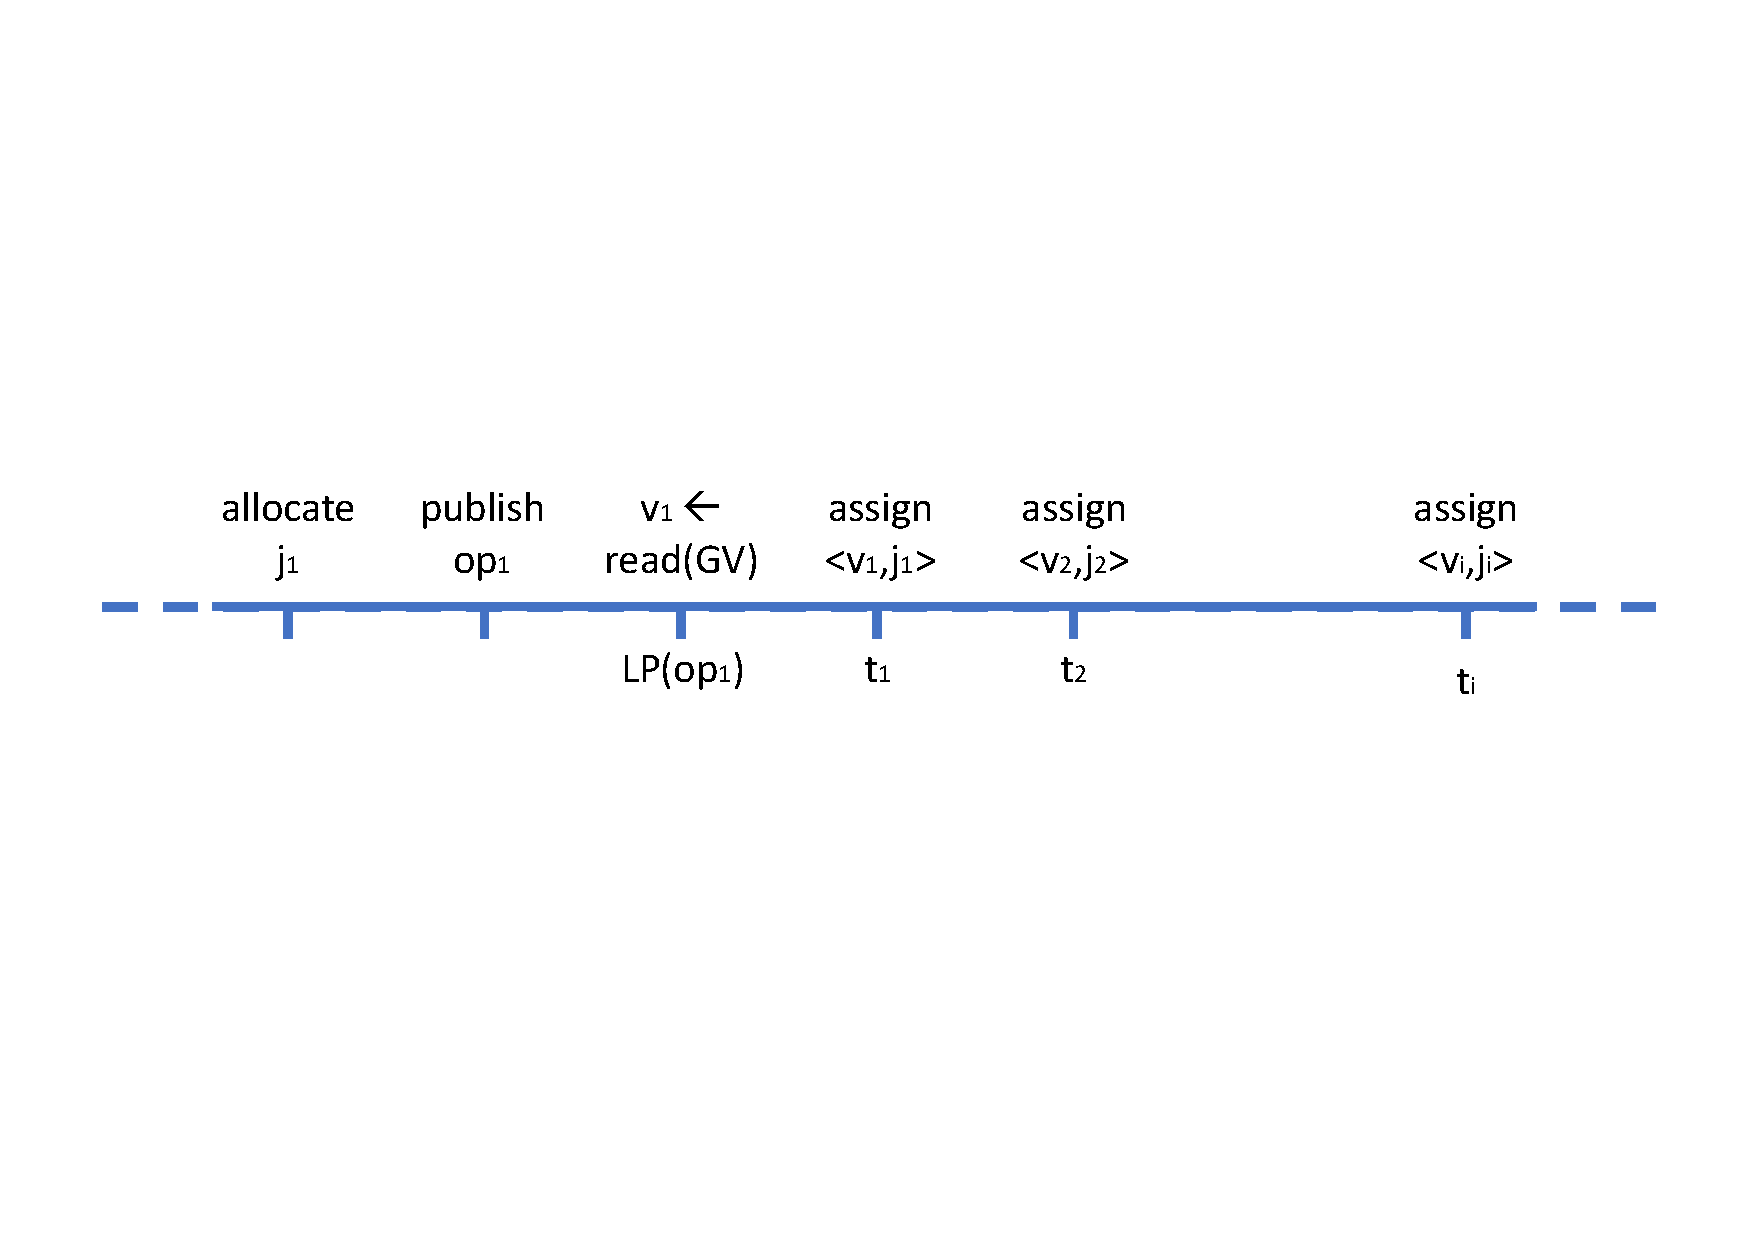
\includegraphics[scale=0.5]{proof-put-base.pdf}
      \caption[]{Base case: ...}
    \label{fig:proof-put-base}  
  \end{subfigure}   \hskip .1\columnwidth
  \begin{subfigure}[t]{1.0\columnwidth}
      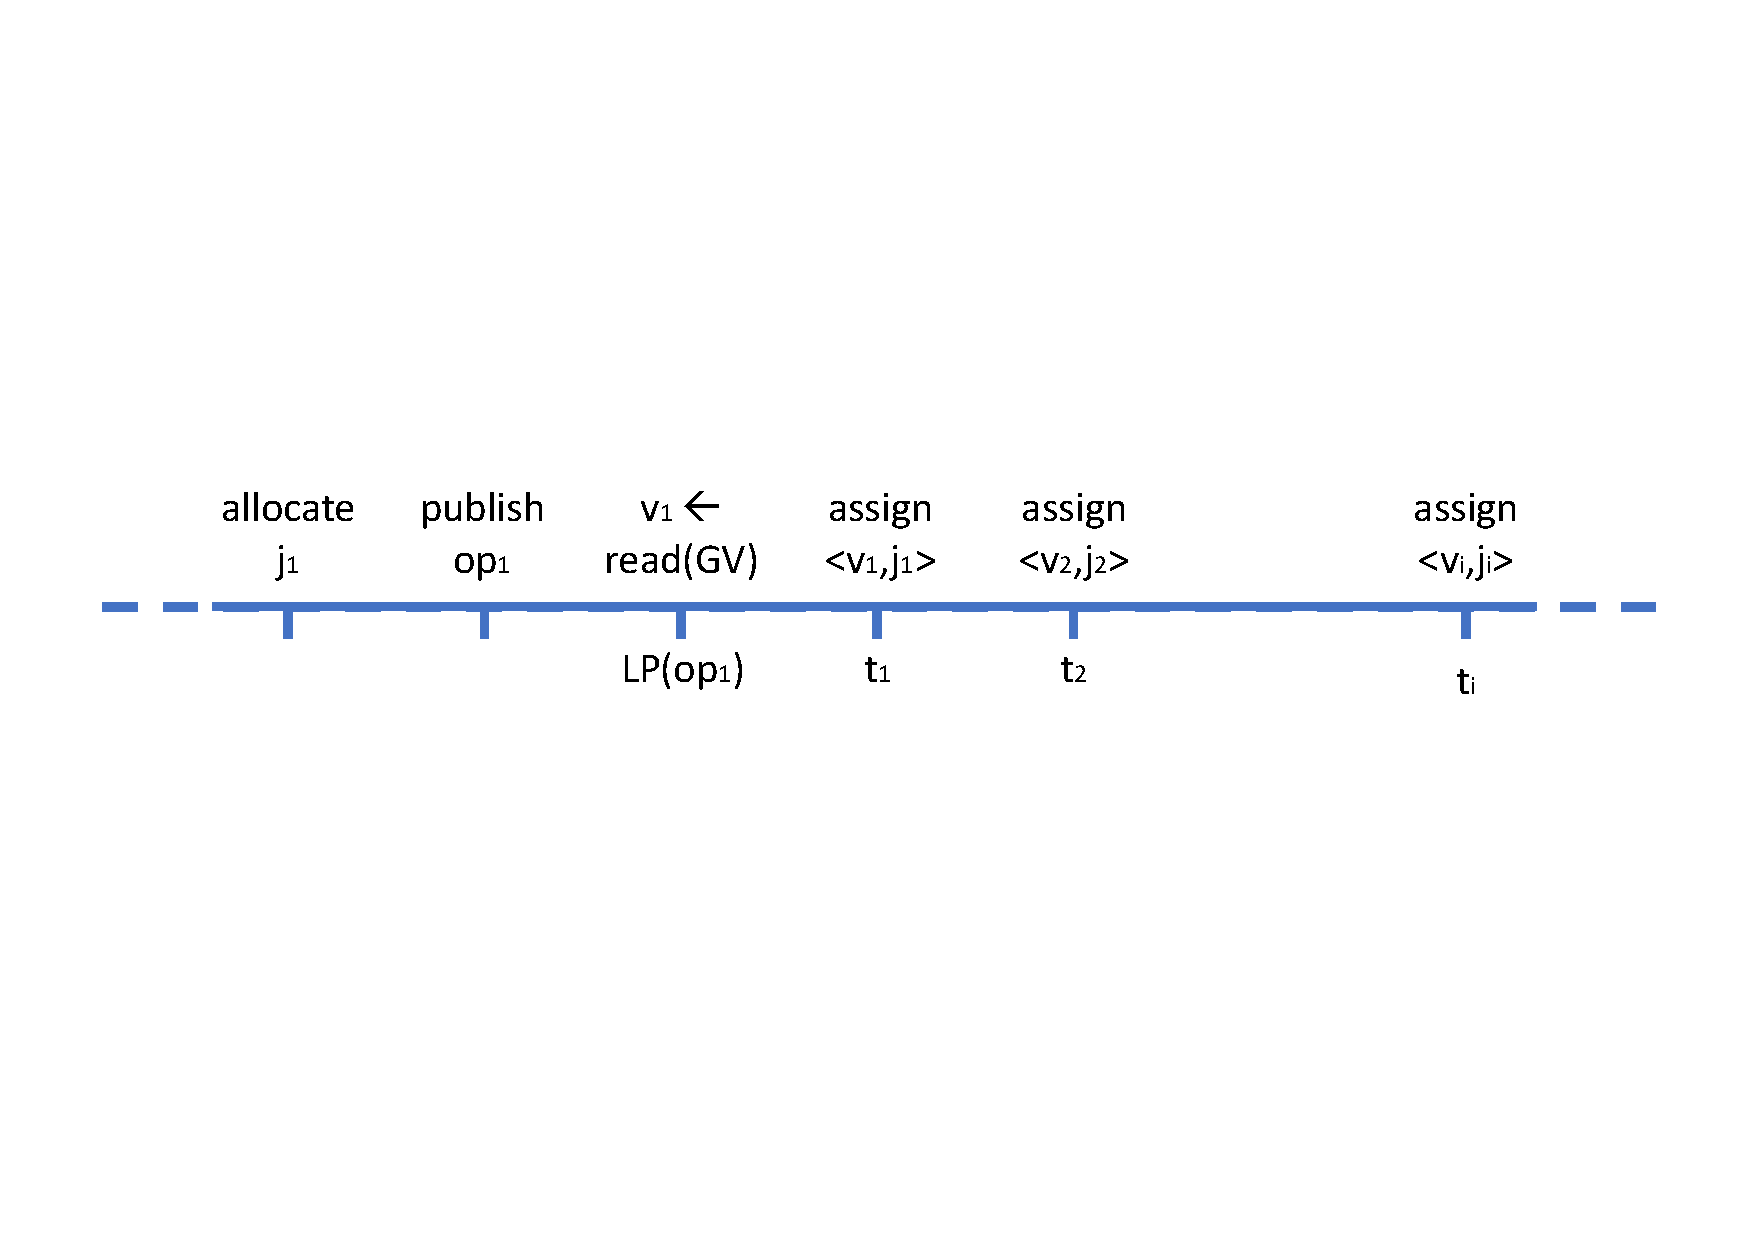
\includegraphics[scale=0.5]{proof-put-base.pdf}
      \caption[]{Induction step: ...}
    \label{fig:proof-put-ind1}
  \end{subfigure}
  \begin{subfigure}[t]{1.0\columnwidth}
      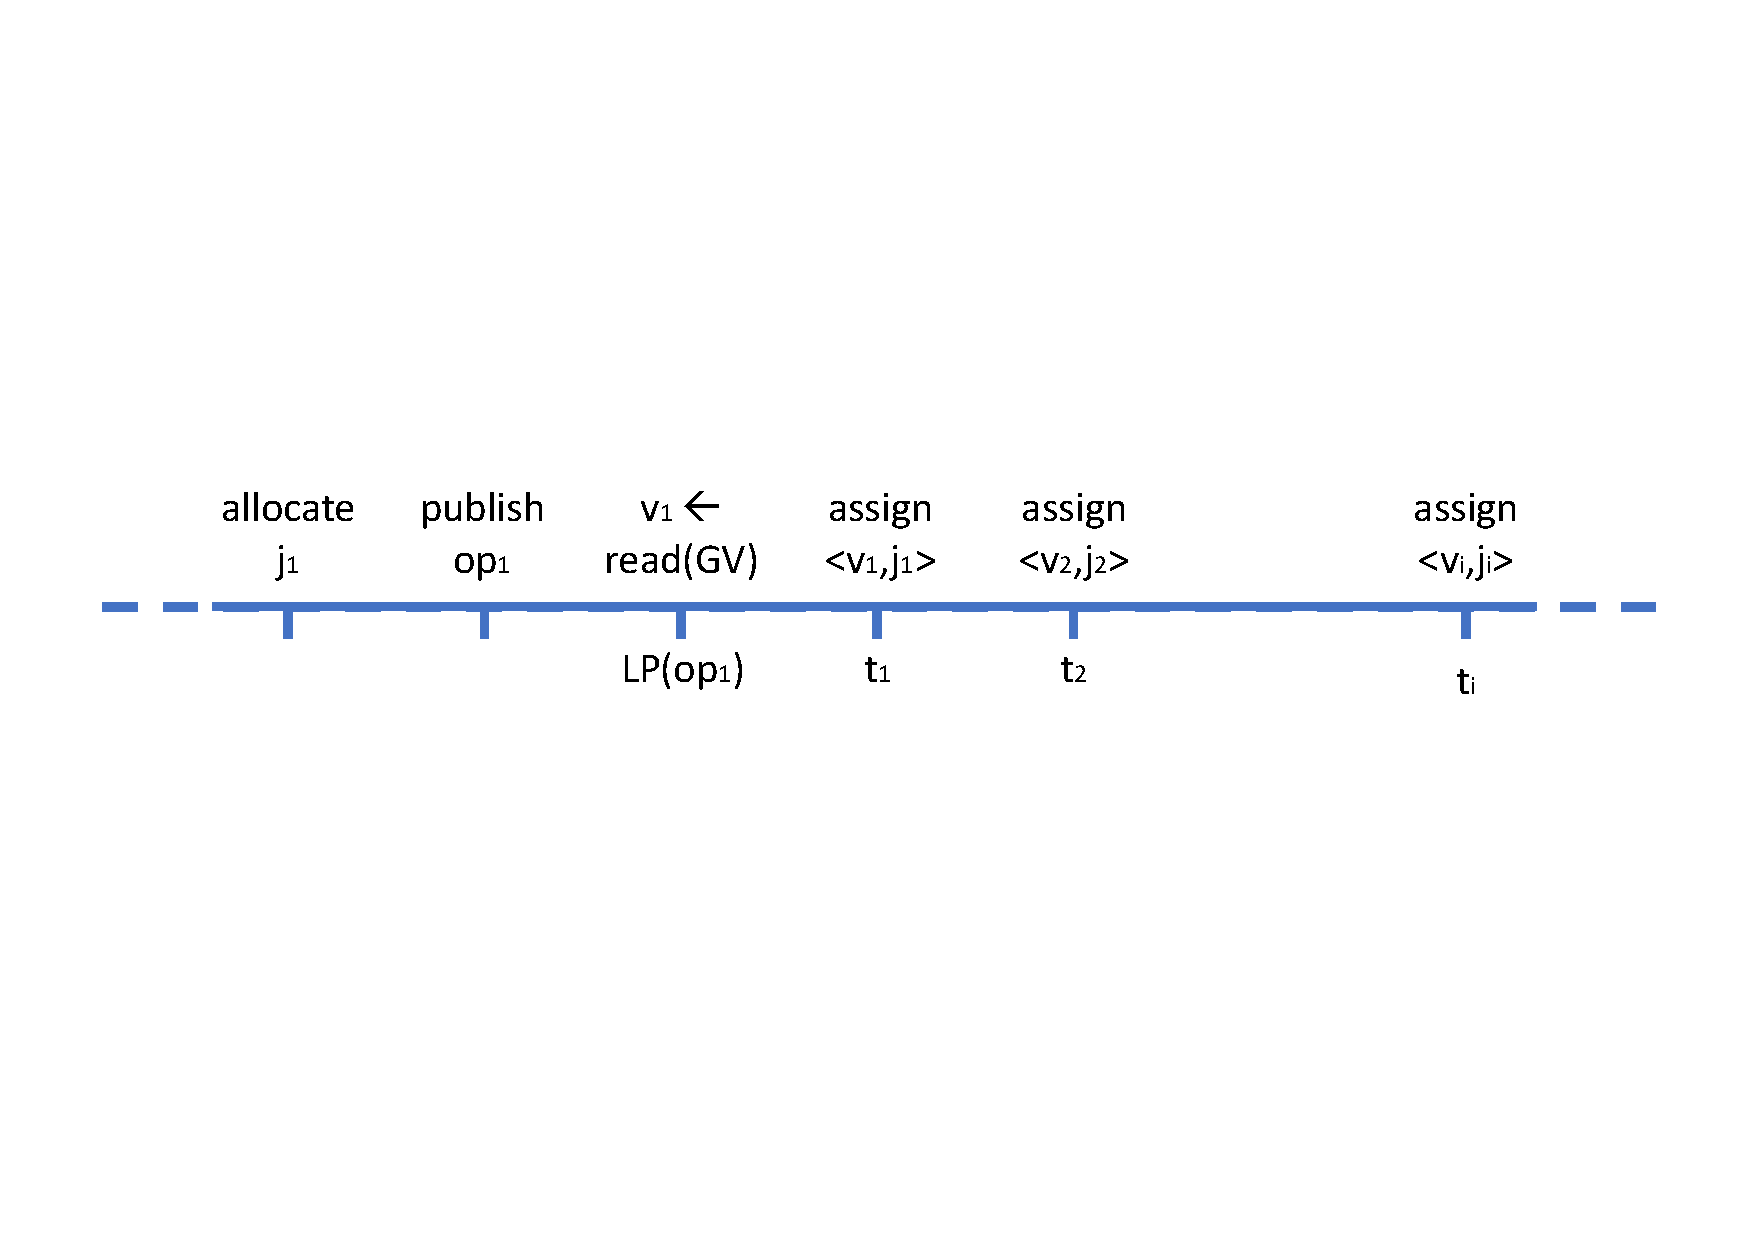
\includegraphics[scale=0.5]{proof-put-base.pdf}
      \caption[]{Induction step: ...}
    \label{fig:proof-put-ind2}
  \end{subfigure}
  \begin{subfigure}[t]{1.0\columnwidth}
      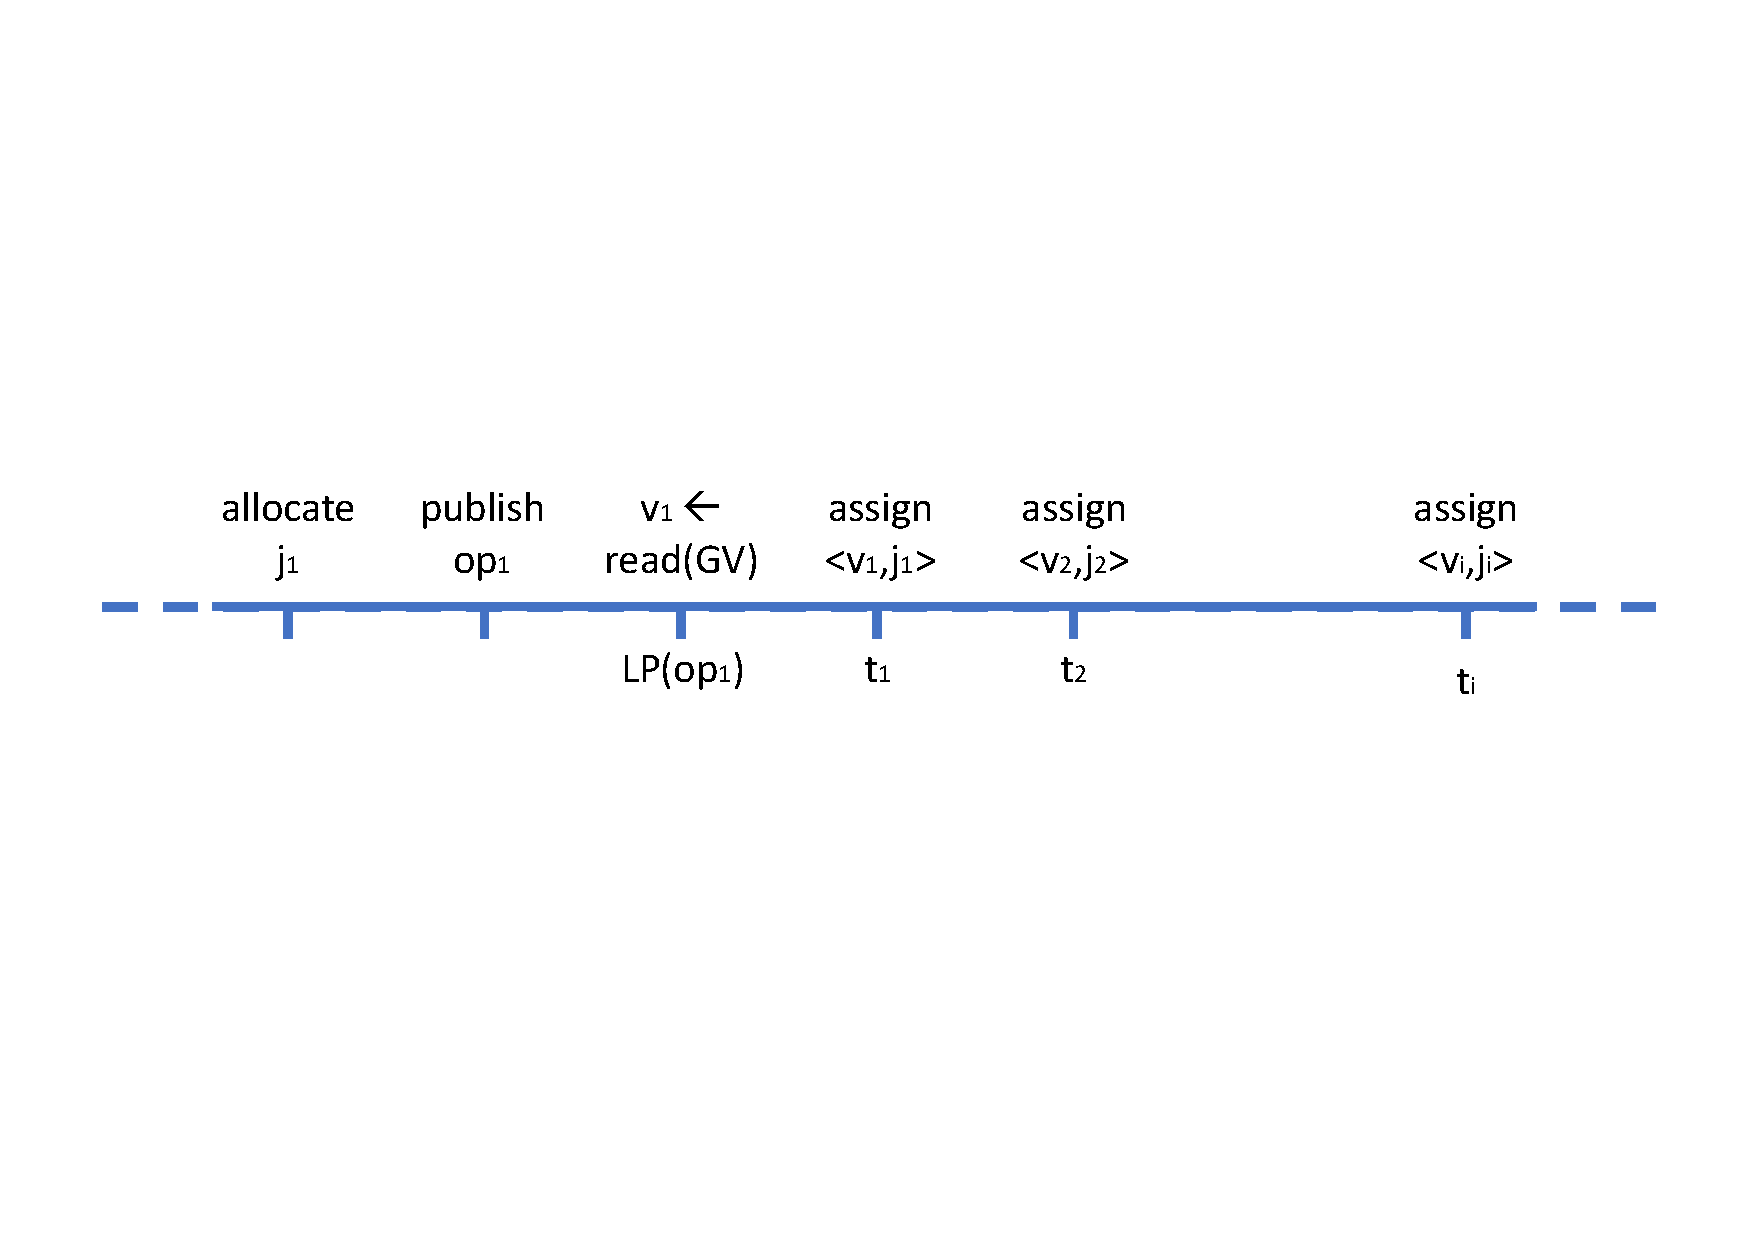
\includegraphics[scale=0.5]{proof-put-base.pdf}
      \caption[]{Induction step: ...}
    \label{fig:proof-put-ind3}
  \end{subfigure}

\caption{Linearization points of put operations. } 
\label{fig:proof-put}
\end{figure*}


\subsubsection{Gets and scans.}
\label{ssec:get-proof}

The most subtle linearization is of get operations.
A get operation $go$ may land in a mutable or immutable chunk. 
We need to linearize $go$ before all concurrent puts that $go$ misses while seeking the value.
%get
For a get operation $go$ for a key $k$ in the range of chunk $C$, we consider the time $t$ when $go$ starts traversing $C$'s PPA (line~\ref{l:get-traversePPA} in \code{helpPendingPuts}). There are three options:
\begin{enumerate}
\setlength{\itemsep}{0pt}
\setlength{\parskip}{0pt}
\item If $C$ is not accessible from the chunks list at time $t$, then \lp{go} is the last step in which $C$ is still accessible from the chunks list.
\item Else, if $go$ does not find $k$ in $C$ then \lp{go} is at time $t$.
\item Else, let $po$ be the put operation that inserts the value returned by $go$. \lp{go} is the latest between time $t$ and immediately after \lp{po}.
\end{enumerate}
\eshcar{ADD FIGURES}

The next lemma shows that in the third case no other put writing to $k$ is linearized after \lp{po} and before \lp{go}.
The proof relies on 
Lemma~\ref{proof:put} and the rebalance invariants.

\begin{lemma}
\label{proof:get}
Consider a get operation $go$ retrieving the value of key $k$ from chunk $C$. Let $t$ be the step in which $go$ starts traversing $C$'s {PPA}. Then:
\begin{enumerate}
\setlength{\itemsep}{0pt}
\setlength{\parskip}{0pt}
\item \label{proof:get:lp1} If $go$ does not find $k$ in $C$, then for each operation $po$ publishing $k$ in $C$, \lp{po} is after $t$.
\item \label{proof:get:lp2} If $go$ returns the value written by operation $po$, then \lp{go} is after \lp{po}, and for each  $po' \neq po$ publishing $k$ in $C$, \lp{po'} is either before \lp{po} or after $t$.
\end{enumerate}
\end{lemma}
\begin{proof}
%It can be inferred from \code{findLatest} that $op$ returns the value with the maximal location-based version observed by $op$ in the \code{ppa} and in the cell linked list. In addition, it can be inferred from the code that put operations update values in-place in the cell linked list only if its full version is higher than the full version of the cell in the list.

First, assume $go$ did not find the key in $C$. It can be inferred from \code{findLatest}, all operations publishing $k$ in $C$ are published in the \code{ppa} after $t$. Otherwise, $go$ should have observed one of them either in the \code{ppa} or in the linked list. By Condition~\ref{proof:put:lp3} of Lemma~\ref{proof:put}, all operations publishing $k$ in $C$ are linearized after $t$, and Condition~\ref{proof:get:lp1} holds.

Next, assume $go$ returns the value written by operation $po_l$, where the full version of $po_l$ is $\langle v_l, j_l\rangle$. 

If $C$ is not accessible from the chunks list at time $t$, then \lp{go} is in the last step in which $C$ is accessible from the chunks list. By the rebalance invariant no put operation can publish in $C$ after $t$, and by Condition~\ref{proof:put:lp1} of Lemma~\ref{proof:put}  \lp{go} is after \lp{po_l}. Otherwise, by definition that \lp{go} is (immediately) after  \lp{po_l}.

Consider an operation $po_m \neq po_l$ publishing $k$ to $C$ with full version $\langle v_m, j_m\rangle$.
By Condition~\ref{proof:put:lp4} of Lemma~\ref{proof:put}, if $\langle v_m, j_m\rangle < \langle v_l, j_l\rangle$ then \lp{po_m} is before \lp{po_l}. It is left to show that if $\langle v_m, j_m\rangle > \langle v_l, j_l\rangle$ then \lp{po_m} is after $t$.
It can be inferred from \code{findLatest}, all operations publishing $k$ in $C$ with full version $\langle v_m, j_m\rangle > \langle v_l, j_l\rangle$ are published in the \code{ppa} after $t$. Otherwise, $go$ should have observed one of them either in the \code{ppa} or in the linked list.
Condition~\ref{proof:put:lp3} of Lemma~\ref{proof:put} implies that these operations are linearized after at least one of them is published in the \code{ppa}, hence Condition~\ref{proof:get:lp2} also holds.
\end{proof}

Scans are linearized when \code{GV} is increased beyond their read point, typically by their own F\&I, and sometimes by a helping rebalance. 
Lemma~\ref{proof:put} helps to prove the following:
\begin{lemma}
\label{proof:scan}
Consider a scan operation $so$ that acquires version $v$ as its read point. For each key $k$ in the range of the scan, $so$ returns the value of the put operation writing to $k$ that is linearized last before \lp{so}.
\end{lemma}
\begin{proof}
%It can be inferred from \code{findLatest} that for each key $k$ in the range of the scan, $op$ returns the maximal location-based version of $k$ that does not exceed the scan read point observed by $op$ in the \code{ppa} and in the cell linked list. In addition, it can be inferred from the code that put operations update values in-place in the cell linked list only if its location-based version is higher than the location-based version of the cell in the list.

Consider a put operation $po$ that writes to a key in the range of the scan but is not observed by $op$. If $po$ acquires version that is less than $v$ then it acquired a version before the scan increased the global version counter. Since $so$ did not observe $po$ in the \code{ppa}, $po$ completed before $so$ read the entry in the \code{ppa}. $so$ did not observe $po$ in the linked list. It can be inferred from the code that another put operation $po'$ with a higher version than $po$'s full version updated the $k$'s value in-place in the linked list.
By Condition~\ref{proof:put:lp4} of Lemma~\ref{proof:put}, $po$ is linearized before $po'$ writing the value returned by the scan.

Finally, by Condition~\ref{proof:put:lp2} of Lemma~\ref{proof:put} all put operations that are not observed by $so$ and acquire version that is greater than $v$ are linearized after \lp{so}.
\end{proof}

The definition of the linearization points of scans and get operations imply that these operations are linearized between their invocation and return.
Condition~\ref{proof:put:lp1} of Lemma~\ref{proof:put} implies the same for puts. 
It is easy to show \eshcar{show it!! before the lemmas} that gets and scans land in chunks that contain the saught keys in their ranges. Combined with the rebalancing invariants,
Lemma~\ref{proof:get} shows that get operations satisfy their sequential specification, and Lemma~\ref{proof:scan} proves that scans satisfy their sequential specification. 
Hence we conclude that \kiwi\ implements a linearziable map. 
